\chapter{Base de Dados e Metodologia}
% \chapter{Metodologia}
% \section{Organização dos Dados e Área de Estudo}

\section{Descrição das Bases de Dados}

\subsection{Departamento de Informática do Sistema Único de Saúde (DataSUS)}

O \acrshort{DataSUS} está inserido atualmente na pasta da Secretaria Executiva do Ministério da Saúde e a \acrfull{Dive} é vinculada à Superintendência de Vigilância em Saúde, da Secretaria de Estado da Saúde de Santa Catarina. O \acrshort{DataSUS} disponibiliza informações, via plataforma TABNET, que subsidiam  análises objetivas da situação sanitária para tomada de decisões baseadas em evidências e elaboração de programas de ações para promoção da saúde \cite{TABNETMinisterio}.

\indent Atualmente, dados como condições de vida, acesso a serviços, qualidade da atenção à saúde, morbidade, incapacidade, além de fatores ambientais, passaram a ser métricas utilizadas na construção de Indicadores de Saúde, que se traduzem em informação relevante para a quantificação e a avaliação das informações em saúde \cite{TABNETMinisterio}.

\subsection{Sistema de Informação de Agravos de Notificação (Sinan)}

\indent O \acrfull{Sinan} foi implantado em 1993, porém apenas em 1998 o \acrfull{Cenepi} coordenou e organizou as três esferas do governo por meio da Portaria \acrshort{Funasa}/Ministério da Saúde n.º 073 de 9/3/98, regulamentando  e tornando obrigatória a alimentação regular dessa base de dados nacional \cite{SINAN07Ministerio}.

\indent A partir de 2003, com a criação do \acrfull{SVS}, essa secretaria passa a ser responsável pelo sistema. Apesar de o \acrshort{Sinan} ser alimentado por notificações  de casos de doenças e agravos que constam da lista nacional de doenças de notificação compulsória, é facultado aos estados e municípios incluir outros agravos de saúde importantes em sua região \cite{SINANWEB, SINAN07Ministerio}.

\indent O próprio \acrshort{Sinan} faz a publicização, em documento ofical ao final do ano, das semanas epidemiológicas do próximo ano. Essas, como mencionado pelo \citeonline{SemanaEpidemio}, foram convencionadas internacionalmente e são contadas a partir de domingo a sábado. "A primeira semana do ano é aquela que contém o maior número de dias de janeiro e a última a que contém o maior número de dias de dezembro."

\indent No ano de 2023, a \acrlong{SVS} passa a ser denominada \acrlong{SVSA}, por incluir a abordagem da Saúde Única dentro do próprio Ministério da Saúde. Tal alteração foi oficializada, inicialmente, pelo Decreto nº 11.358 de 1º de janeiro; posteriormente revogado e vigente sob o Decreto nº 11.798 de 28 de novembro \cite{SVSA2023_1, SVSA2023_2}.

\subsection{Vigilantos}

O Vigilantos é o sistema informatizado \ingles{on-line} desenvolvido em 2012 pelo Estado de \acrlong{SC}. Os municípios podem inserir dados relativos ao \latim{Aedes aegypti}, facilitando e agilizando o acesso de todos os níveis a essa informação. Além de permitir registro, é possível fazer análise das informações de vigilância e controle vetorial através de dois módulos: Módulo Focos e Módulo Programa de Controle da Dengue \cite{Vigilantos}.

\subsection{Malhas Territoriais}

Em relação aos dados georreferenciados, são disponibilizados como malhas territoriais pelo \acrfull{IBGE} das três esferas, seja Federação, Unidade Federativa ou Município. Pode ser conferido no seguinte endereço eletrônico:
\begin{center}
\url{https://www.ibge.gov.br/geociencias/organizacao-do-territorio/malhas-territoriais/}. %15774-malhas.html
\end{center}

O \acrshort{IBGE} tem como missão, resumidamente: identificar e analisar o território; realizar a contagem da população; mostrar como a economia evolui através do trabalho e da produção das pessoas, revelando ainda como elas vivem.  O Instituto é o principal provedor de dados e informações do Brasil, que atendem às necessidades da sociedade civil, assim como dos órgãos das esferas governamentais federal, estadual e municipal \cite{IBGE22, IBGE23prev}. 

% \subsection{Banco de Dados Meteorológicos do Instituto Nacional de Meteorologia (Bdmep/Inmet)}

% O \acrshort{Bdmep/Inmet} reune dados meteorológicos diários em formato digital, sendo atualizados a cada 90 dias e disponibilizados via \ingles{internet}. Essas séries históricas foram coletadas das várias estações meteorológicas convencionais da rede de estações do próprio \citeonline{INMET22}, que está vinculado diretamente ao \acrfull{MAPA}.

\subsection{\ingles{Merging Technique (MERGE)}}

\indent De acordo com \citeonline{Rozante2010MERGE} o produto \acrshort{MERGE} é a combinação, através de métodos estatísticos, de dados do satélite \ingles{\acrfull{TRMM-TMPA}} e a precipitação observada por estações de superfície. Esse produto é de alta resolução espacial (0.1º), com gradeamento de 10km² e disponibilização de dados diários a partir de junho de 2000, e horários desde 2010.

\indent Comentado por \citeonline{IMERG, TRMM-TMPA}, os dados do \ingles{\acrshort{TRMM-TMPA}} foram descontinuados e é fortemente sugerido utilizar dados do \ingles{\acrfull{GPM-IMERG}}. Esses dados são disponibilizados a cada 30 minutos e as estimativas são executadas em duas etapas: antecipada (\ingles{Early}) e tardia (\ingles{Late}). A estimativa \ingles{Early} tem atraso de apenas quatro horas e é compilada com dados do momento. Por outro lado, a estimativa \ingles{Late} tem atraso de 12 horas e é compilada com mais dados, o que a torna mais precisa.

\indent Atualmente, o produto \ingles{\acrshort{MERGE}} já faz a interpolação das observações das estações de superfície com dados do \ingles{\acrshort{GPM-IMERG}-Late} (figura \ref{fig:merge_obs24}). Essa atualização do \ingles{\acrshort{MERGE}} tem a inclusão de aproximadamente 2500 dados observados (figura \ref{fig:obs_prec24}) e a exlusão de Viés das estimativas de precipitação por modelos satelitais, em comparação à versão anterior \cite{MERGEatual}

\indent O produto é gerado e disponibilizado (figura \ref{fig:merge24}) operacionalmente pelo \acrshort{CPTEC}/\acrshort{INPE}, no formato \ingles{\acrfull{grib} (.grib2)}. Estão disponíveis dados horários, diários e climatológicos de precipitação, podendo ser acessados pelo seguinte endereço eletrônico: \url{http://ftp.cptec.inpe.br/modelos/tempo/MERGE/}.

\begin{figure}[htbp]
    \centering
    \caption{Produto \ingles{MERGE} e estações meteorológicas usadas na interpolação. Visualização dos dados durante o solstício de inverno de 2024.} %LEGENDA DA IMAGEM GLOBAL
    \label{fig:merge_obs24}
    \subfloat[Número estações meteorológicas disponíveis na América do Sul para interpolação do produto. \label{fig:obs_prec24}]{
    \includegraphics[width = 0.45 \textwidth]{PREC_OBS_20240620.png}
    }\hfill
    \subfloat[Produto \ingles{MERGE} no tamanho original, disponível para a América do Sul. \label{fig:merge24}]{
    \includegraphics[width = 0.45 \textwidth]{MERGE_DAILY_20240620.png}
    }\\
    \small{Fonte: \acrshort{CPTEC}/\acrshort{INPE}, \citeauthor{MERGEatual} (2024).}
\end{figure}

\subsection{\ingles{South American Mapping of Temperature (SAMeT)}}

\indent O produto \ingles{\acrshort{SAMeT}} também é de alta resolução espacial (0,05º), com gradeamento de 5km² e sendo a interpolação de estimativas do modelo \ingles{\acrfull{ERA5}} [\ingles{\acrfull{ECMWF}}] e regressão linear simples com \ingles{\acrfull{GTOPO30}}, além de observações de estações (convencionais e automáticas) de temperatura a 2 metros (figura \ref{fig:samet_obs24}).
 
\indent Pelo fato de a reanálise ter atraso de cinco dias, o produto é inicialmente gerado com dados de observação e com modelos numéricos de previsão. Assim que a reanálise se torna disponível, o produto é gerado novamente com dados integrais da reanálise (modelo \ingles{\acrshort{ERA5}}) interpolados a dados de estações meteorológicas (figura \ref{fig:obs_temp24}). Essa combinação, entre reanálise e observação, traz uma acurácia maior ao produto, principalmente em locais de acentuada topografia \cite{Rozante2021SAMeT}.

\indent O produto é gerado e disponibilizado (figura \ref{fig:samet24}) operacionalmente pelo \acrshort{CPTEC}/\acrshort{INPE}, no formato \ingles{\acrfull{nc} (.nc)}. Estão disponíveis dados diários e climatológicos de temperaturas mínima, média e máxima, podendo ser acessados pelo seguinte endereço eletrônico: \url{http://ftp.cptec.inpe.br/modelos/tempo/SAMeT/}.

\begin{figure}[htbp]
    \centering
    \caption{Produto \ingles{SAMeT} e estações meteorológicas usadas na interpolação. Visualização dos dados durante o solstício de inverno de 2024.} %LEGENDA DA IMAGEM GLOBAL
    \label{fig:samet_obs24}
    \subfloat[Número estações meteorológicas disponíveis na América do Sul para interpolação do produto. \label{fig:obs_temp24}]{
    \includegraphics[width = 0.45 \textwidth]{TMIN_OBS_20240620.png}
    }\hfill
    \subfloat[Produto \ingles{SAMeT} no tamanho original, disponível para a América do Sul. \label{fig:samet24}]{
    \includegraphics[width = 0.45 \textwidth]{SAMeT_TMIN_20240620.png}
    }\\
    \small{Fonte: \acrshort{CPTEC}/\acrshort{INPE}, \citeauthor{Rozante2021SAMeT} (2024).}
\end{figure}

\subsection{\ingles{Global Forecast System (GFS)}}

\indent Segundo a Administração Oceânica e Atmosférica Nacional (estadunidense) \citeyear{GFS} (\ingles{\acrfull{NOAA}}), o modelo \ingles{\acrshort{GFS}} é a regressão da reanálise do modelo \ingles{\acrfull{MERRA2}}; e atualizado para a versão 16.0 (\ingles{\acrshort{GFS}v16}) em março de 2020. Os dados são disponibilizados quatro vezes ao dia (00, 06, 12 e 18 UTC), com até 16 dias de previsão, tendo variações: dados horários para até os primeiros cinco dias (0,25º) e dados a cada três horas para até 16 dias (0,5º).

\indent Para \citeonline{GFSart}, a versão 15 do \acrshort{GFS} ficou disponível após a troca do componente principal do modelo, anteriormente baseado no Modelo Espectral Global (\ingles{\acrfull{GSM}}), pelo Núcleo Dinâmico Cúbico de Volumes Finitos (\ingles{\acrfull{FV3}}). Como descrito por \citeonline{GFSart2}, a atualização para versão 16 ocorreu após a inclusão de mais camadas verticais e atualizações nos modelos físicos. 

\indent Esse modelo preditivo é sintetizado pelo Centro Nacional para Previsões Ambientais daquele mesmo país (\ingles{\acrfull{NCEP}}), que faz acoplamento de quatro outros modelos (atmosférico, oceanográfico, terrestre e de gelo marinho), retornando valores preditivos de temperaturas, precipitação, umidade relativa do ar e do solo, radiação, relativas ao vento, assim como concentração de ozônio \cite{GFS24NOAA}.

\section{Conjunto de Dados e Área de Estudo}

\indent As informações epidemiológicas (casos de dengue) e entomológicas (focos de \latim{Aedes} sp.) foram obtidas através de dados oficiais do Ministério da Saúde / \acrfull{SVSA} / \acrfull{Dive}, através de plataformas \ingles{on-line} TabNet-\acrshort{Sinan} (\acrshort{DataSUS} [\url{http://tabnet.datasus.gov.br/cgi/deftohtm.exe?sinannet/cnv/denguebsc.def}] e \acrshort{Dive} [\url{http://tabnet.dive.sc.gov.br/}]) e disponibilizados oficialmente (\acrshort{Dive}).

\indent Os dados referentes a focos de \latim{Aedes} sp. são disponibilizados pela \acrshort{Dive} como arquivos tabulados em planilhas eletrônicas (formato .xls) obtidos a partir de relatórios de número de focos. Esses números são contabilizados no dia do próprio registro, ocorrendo apenas de segunda a sexta-feira. A série histórica desses dados entomológicos tem início no ano de 2012.

\indent Sobre os dados de casos de dengue, obtidos \ingles{online} do TabNet \acrshort{Sinan}, sendo selecionados: Município de Infecção e Semana Epidemiológica do início dos Sintomas [sic], assim como refinar os dados com confirmação Laboratorial e Clínico-epidemiológica, além de incluir todas as nomenclaturas de registro para a dengue (Dengue com complicações, Febre Hemorrágica do Dengue, Síndrome do Choque do Dengue, Dengue, Dengue com sinais de alarme, Dengre [sic] grave).  A série histórica dos casos de dengue começa em 2014, sendo previamente agrupados e já disponibilizados em semanas epidemiológicas.

\indent Também foram utilizados dados georreferenciados atualizados do (\acrfull{IBGE}). Sobre elementos climáticos, os dados são de:
i) Precipitação e temperatura - fornecidos pelo \ingles{\acrfull{GFS}}; ii) Precipitação - obtido pelo produto \ingles{\acrfull{MERGE}} e iii) Temperatura - obtido pelo produto \ingles{\acrfull{SAMeT}}.
% \begin{itemize}
%     \item Precipitação e temperatura - fornecidos pelo \ingles{\acrfull{GFS}};
%     \item Precipitação - obtido pelo produto \ingles{\acrfull{MERGE}};
%     \item Temperatura - obtido pelo produto \ingles{\acrfull{SAMeT}}.
% \end{itemize}


\indent Em relação à precipitação acumulada na superfície (mm), provenientes do produto \ingles{\acrshort{MERGE}}, foram adquiridos dados diários a partir de junho de 2000 e com resolução de 10 km² (0,1º).

\indent Os dados de temperatura (\ingles{\acrshort{SAMeT}}) são aferidos a dois metros (2m) da superfície em escala de temperaturas dadas em celsius (C), agrupados em médias diárias, com a série histórica iniciando em janeiro de 2000 e com resolução de 5 km² (0,05º).

Para organização, os dados serão agrupados em três divisões distintas: 

\begin{alineas}

    \item \acrfull{DEE}: Elementos sanitários relacionados tanto ao vetor (dados entomológicos) quanto ao hospedeiro (dados epidemiológicos) e provenientes de bancos de dados oficiais. Os valores são relativos à quantidade de focos de \latim{Aedes} sp., disponibilizados oficialmente pela \acrshort{Dive}. Em relação à quantidade de casos de dengue, esses dados foram obtidos de plataformas \ingles{on-line}: TABNET-\acrshort{Sinan}-\acrshort{DataSUS} (base nacional) e TABNET-\acrshort{Sinan}-\acrshort{Dive} (base estadual);
    
    \item \acrfull{DEC}: Informações referentes a variáveis meteorológicas/climatológicas (temperatura - mínima, máxima e média - e precipitação) e provenientes de banco de dados oficiais (reanálise e produtos de reanálise):  \ingles{\acrshort{GFS}}, \ingles{\acrshort{MERGE}} e \ingles{\acrshort{SAMeT}};

    \item \acrfull{DGR}: Informações relacionadas aos aspectos geográficos atualizados para o momento atual, provenientes do \acrshort{IBGE}. 
    
\end{alineas}

\indent Os \acrshort{DEE} e \acrshort{DEC} foram estruturados a ponto de compartilhar a mesma escala espaço-temporal. Os dados diários foram agrupados em semanas epidemiológicas, segundo convenção internacional citada por \citeonline{SemanaEpidemio}, assim como o recorte espacial englobou área de estudo (figura \ref{fig:area_de_estudo}), o próprio Estado catarinense.

\begin{figure}[htbp]
    \centering
    \caption{Mapa temático da área de estudo do projeto evidenciando municípios catarinenses.}
    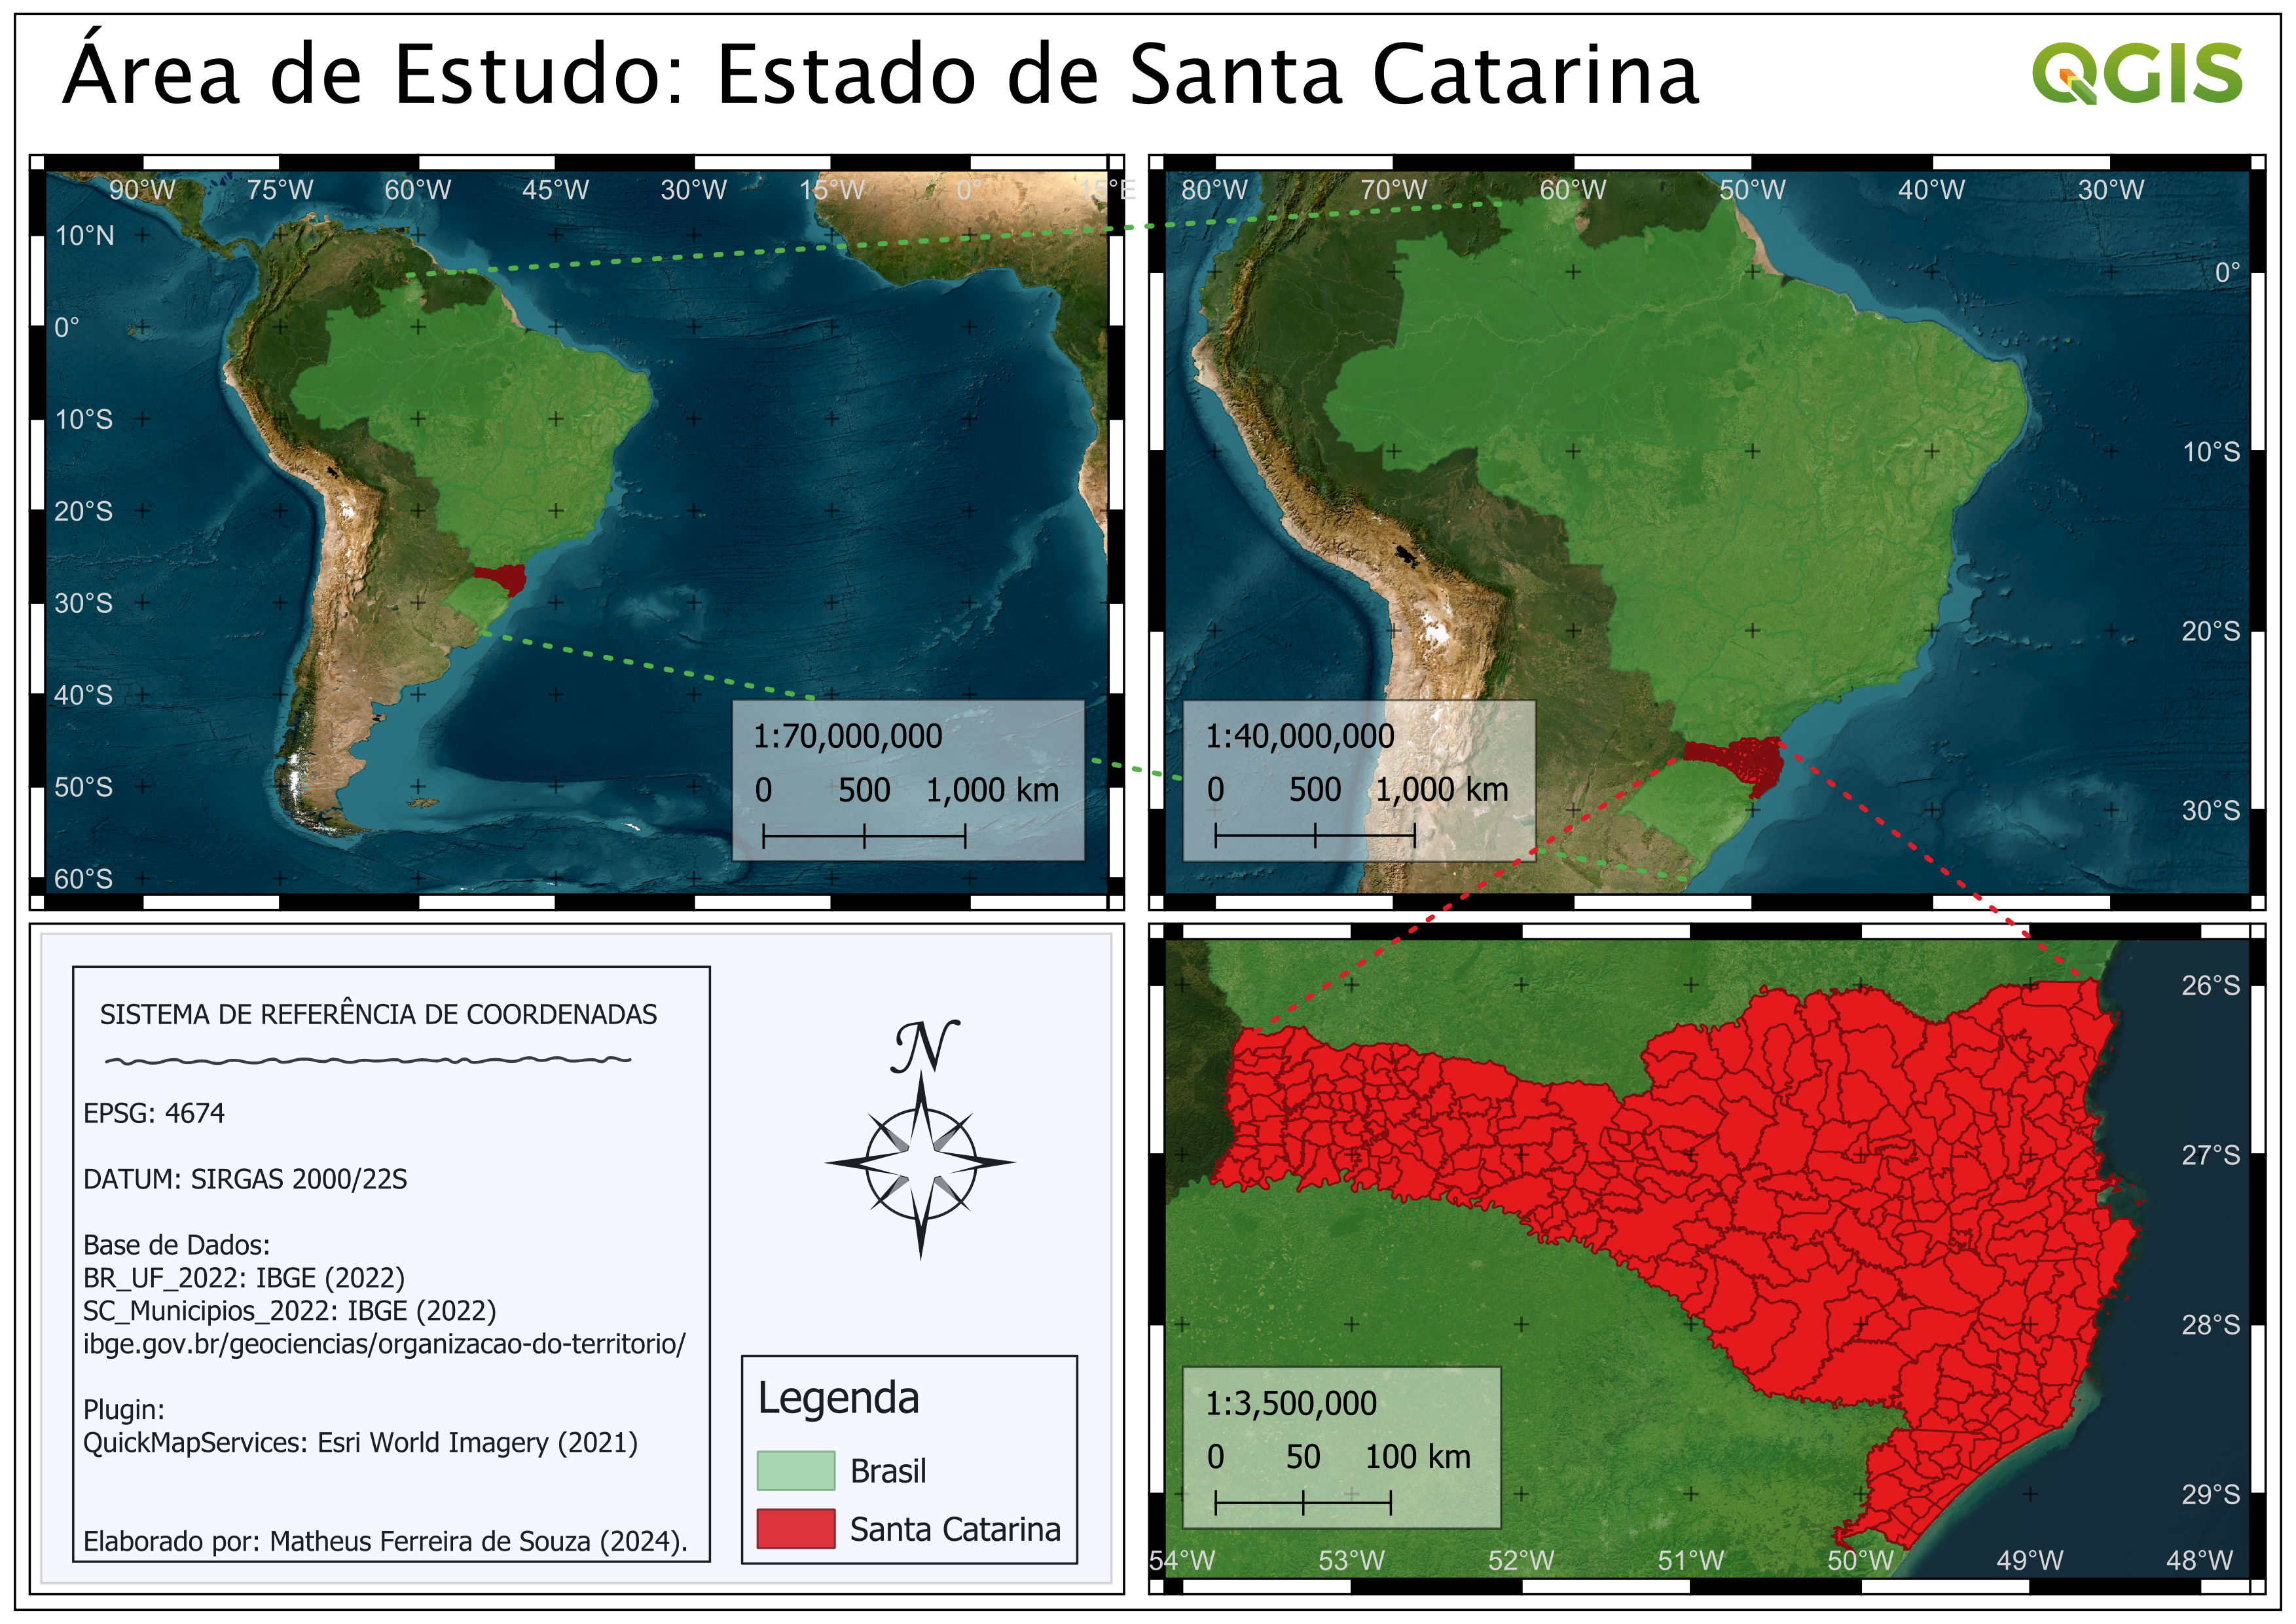
\includegraphics[scale=0.35]{figuras/area_de_estudo_SC_MATHEUS.png}
    \label{fig:area_de_estudo}
    \\
    \vspace{-0.05cm}\hspace{-7.5cm}\small{Fonte: Elaboração própria (2024).} 
\end{figure}

\indent Para melhor explicação dos métodos, pretende-se dividir o estudo em etapas, relativas ao percurso de execução do próprio projeto (figura \ref{fig: fluxograma}), sendo: pré-processamento dos dados; análise climatológica descritiva, do Estado de \acrlong{SC} e de alguns municípios; modelagem preditiva; validação do modelo; espacialização dos dados preditos; além de síntese do \acrfull{PTT}.

\begin{figure}[htbp]
    \centering
    \caption{Fluxograma representando etapas presentes no projeto, contemplando do início (dados brutos) ao final (resultados).}
    \includegraphics[scale=0.6]{figuras/fluxograma_dados.png}
    \label{fig: fluxograma}
    \\
    \vspace{-0.05cm}\hspace{-7.5cm}\small{Fonte: Elaboração própria (2024).} 
\end{figure}

\subsection{Pré-processamento}

Em relação aos \acrshort{DEE}, devem ser orientados ao modo que possam ser concatenados, adicionados, uma planilha após a outra. Utilizou-se a biblioteca \ingles{pandas} da linguagem \ingles{Python} versão 3, como pacote principal para estruturação dos dados. Outras bibliotecas também foram utilizadas, como: \ingles{numpy}, para tratar dados faltantes e tipagem de variáveis; \ingles{datetime} \cite{python2_1995_van}, para padronização de todas as datas e variáveis desse tipo; e \ingles{geopandas}, para manipular arquivos georreferenciados, extrair deles a nomenclatura padrão dos municípios do \acrshort{IBGE} e aplicar aos próprios dados (figura \ref{fig: fluxograma} - item 2 e figura \ref{fig: preprocessamento}).

\begin{figure}[htbp]
    \centering
    \caption{Diagrama representando parte do pré-processamento, principalmente em organização dos dados e padronização dos nomes de municípios.}
    \includegraphics[scale=0.7]{figuras/preprocessamento.png}
    \label{fig: preprocessamento}
    \\
    \vspace{-0.05cm}\hspace{-7.5cm}\small{Fonte: Elaboração própria (2024).} 
\end{figure}

\indent Os \acrshort{DEC} foram previamente convertidos de formato \ingles{\acrshort{grib}} para formato \ingles{\acrshort{nc}}, por meio de \ingles{script} escrito em linguagem \ingles{shell} \cite{shell_1999_heroldlinux, bash_2007_gnu-free}. Após isso, foram tratados utilizando o \ingles{\acrfull{CDO}} \cite{CDO_2023_schulzweida}, assim, pôde-se unir dados diários para composição de meses e anos, por fim, sintetizando a série histórica. Com esse mesmo \ingles{software} se fez o primeiro recorte espacial (entre longitudes sul 63 e 45, e latitudes oeste 37 e 19), para o sul do Brasil (figura \ref{fig: sul_brasil}), diminuindo o tamanho do arquivo principal. Para abertura e manipulação dos arquivos climáticos, na extensão \ingles{\acrshort{nc} (.nc)}, utilizou-se a biblioteca \ingles{xarray} \cite{xarray_2016_v0_8_0, xarray_2017_hoyer}.

\begin{figure}[htbp]
    \centering
    \caption{Mapa evidenciando o recorte espacial dos dados relacionados à região sul do brasil. Visualização dos dados de temperatura mínima durante o solstício de inverno de 2023.}
    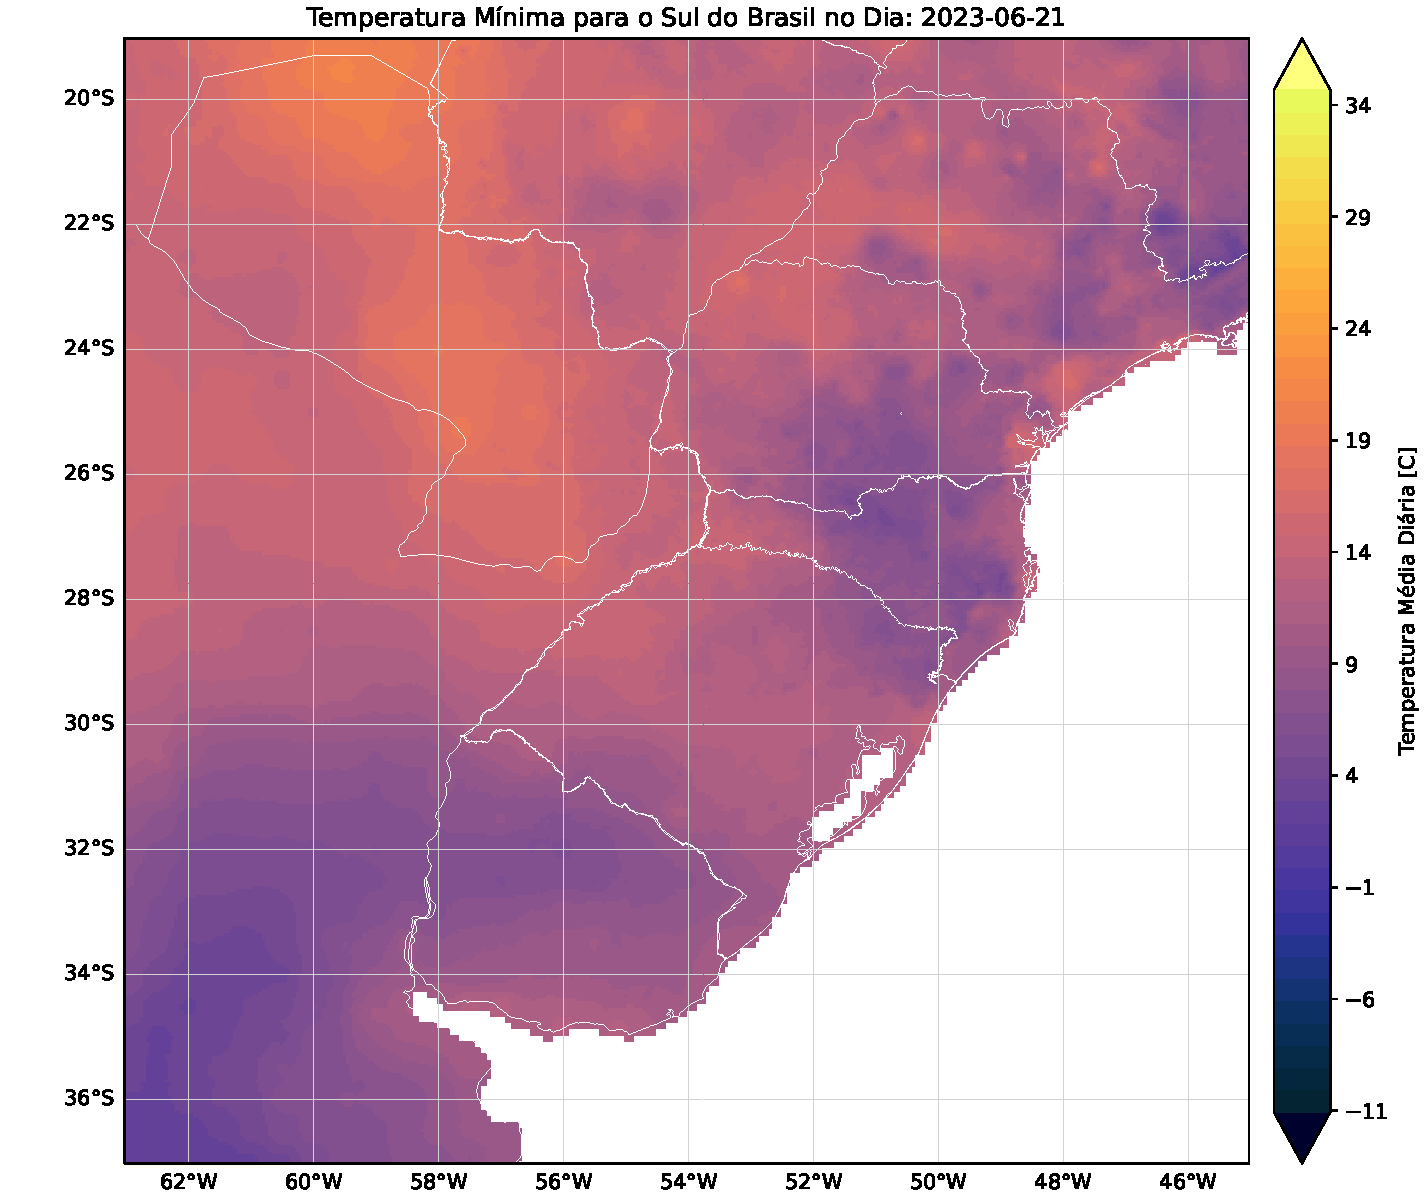
\includegraphics[scale=0.6]{climatologia_tmin_2023-06-21.pdf}
    \label{fig: sul_brasil}
    \\
    \vspace{-0.05cm}\hspace{-7.5cm}\small{Fonte: Elaboração própria (2024).} 
\end{figure}

\indent Após isso, foram extrapolados os valores dos elementos climáticos do centroide de cada município e armazenados em um novo formato de arquivo, \ingles{\acrfull{csv}} (valores separados por vírgulas), utilizando as bibliotecas \ingles{pandas}, \ingles{numpy}, \ingles{geopandas} e \ingles{shapely} \cite{shapely_2007_gillies}.

\indent Finalmente,  os principais conjuntos de dados (temperatura mínima, temperatura média, temperatura máxima, precipitação, focos de \latim{Aedes} sp. e casos de dengue) eram próprios arquivos estruturados em tabela dinâmica, onde as colunas eram cada município catarinense e as linhas, a série histórica dada em semanas epidemiológicas no formato \ingles{datetime64[ns](YYYY-mm-dd)}. Logo, a equiparação entre essas variáveis era possível.

\indent Assim, o presente estudo realiza as análises descritiva e diagnóstica dos elementos climáticos e entomo-epidemiológicos,  análise preditiva dos focos de \latim{Aedes} sp. e casos de dengue e, através deste projeto, cabe aos tomadores de decisão a realização da análise prescritiva.

\section{Análise Descritiva}

\subsection{Análise Climatológica Espacial}

\indent Nessa etapa da metodologia, utilizou-se a linguagem \ingles{Python} (versão 3) \cite{python3_2009_van} para realizar o pré-processamento dos dados (figura \ref{fig: fluxograma} - item 2), comentado à frente, para estruturação básica dos mesmos. Realizou-se a decomposição sazonal dos dados para avaliar tendência na série histórica através da biblioteca \ingles{statsmodels} \cite{statsmodels_2010_seabold}. Para aprofundamento, utilizou-se o teste sazonal de Mann-Kendall , que pondera a sazonalidade dos dados, da biblioteca \ingles{pyMannKendall} \cite{pyMannKendall_2019_Hussain}.

\indent Também, como visualização da distribuição dos dados, fez-se o histograma das séries históricas, através da biblioteca \ingles{matplolib} \cite{matplotlib_2007_hunter}. Com a utilização das bibliotecas \ingles{pandas} \cite{pandas_2010_scipy, pandas_2020_reback} e \ingles{numpy} \cite{numpy_2020_harrisarray}, os menores e maiores valores para os \acrshort{DEC} do Estado catarinense foram encontrados, assim como valores médios e o maior desvio padrão para esses mesmos dados.

\indent Após isso, como as séries históricas dos \acrshort{DEE} e \acrshort{DEC}, foram derivados em novos arquivos. Dessa maneira, cada variável obteve três novas derivações: apenas sazonalidade, série sem sazonalidade e anomalia estacionária (figura \ref{fig: fluxograma} - item 4). 

\indent Esse tratamento foi possível pela biblioteca \ingles{pandas}, extraindo da série o conjunto de semanas epidemiológicas e realizando a média de cada semana ao longo dos anos. Logo, foi subtraído da série histórica o valor sazonal de cada semana epidemiológica, retornando uma série sem sazonalidade.

\indent Por fim, dessa série histórica sem sazonalidade foi subtraída a linha de tendência, utilizando a própria biblioteca  \ingles{pyMannKendall} para acessar o intercepto e o coeficiente angular. Melhor exemplificado na equação abaixo:
\begin{equation}
\indent SAE = SSS - ( a + b * x )
\end{equation}

Onde, a variável $a$ equivale ao intercepto e $b$, ao coeficiente linear. Assim, a \acrfull{SAE} é calculada a partir da \acrfull{SSS}, de onde se subtrai a tendência (obtida pela reta: $a + b * x$).


\indent As matrizes de dados brutos e derivados foram analisadas, podendo-se distribuí-las graficamente no tempo e no espaço. Para isso, as bibliotecas \ingles{matplolib}, \ingles{seaborn} \cite{seaborn_2021_waskom}, \ingles{pandas} e \ingles{geopandas} \cite{geopandas_2020_kelseyjordahl} foram utilizadas.

\subsection{Análise Climatológica de Municípios Selecionados}

\indent Com os mesmos arquivos derivados obtidos na seção anterior, pode-se visualizar graficamente para melhor analisar comportamentos sazonais dos municípios catarinenses selecionados, sendo eles: Florianópolis, Itajaí, Joinville e Chapecó. Esses municípios foram eleitos por apresentarem frequência e volume de dados, além de representarem municípios populosos e distintos. Também, discutido mais a frente, há regionalização nos comportamentos entomo-epidemiológico e climatológico.

\indent Para isso, foi necessário utilizar as bibliotecas \ingles{pandas}, \ingles{matplolib} e \ingles{seaborn}, assim como selecionar apenas as variáveis dos municípios em questão.

\section{Modelagem Preditiva}

\subsection{Análise de Correlações}

\indent Com os conjuntos de dados previamente estruturados, os quatro (4) municípios foram elencados para realizar análises de correlações. Os \acrfull{DEE} (focos de \latim{Aedes} sp. e casos de dengue) e  \acrfull{DEC} (precipitação e temperaturas mínima, média e máxima) foram retroagidos em semanas epidemiológicas para melhor evidenciar possíveis correlações (figura \ref{fig: processamento}). Essas análises foram realizadas entre os \acrshort{DEE} e com os \acrshort{DEC}, assim como entre os \acrshort{DEE} e limiares dos \acrshort{DEC}. 

\indent Os valores dos limiares, calculados a partir da análise climatológica e revisão de literatura, são apresentados no capítulo \ref{Resultados e Discussão} (Resultados e Discussão). Para os limiares de temperatura mínima, foi calculado a partir da média da própria temperatura mínima, selecionando dias que apresentavam valores acima desse limiar média. Os próximos limiares da temperatura mínima foram acrescidos de dois graus Celsius (2 C), totalizando seis (6) limiares de temperatura mínima (C): valores acima de 14, 16, 18, 20, 22 e 24.

\indent Os limiares de temperatura máxima foram estabelecidos em literatura, que considera intervalo entre 22 C e 32 C como ótimo desenvolvimento do vetor \cite{AedesTemp}. Assim, o limiar de temperatura máxima apresenta dias abaixo do limite superior do intervalo encontrado, decrescendo dois graus Celsius (2 C) até atingir um total de seis (6) limiares de temperatura máxima (C), sendo: 22, 24, 26, 28, 30 e 32.

\indent A precipitação, por ser uma variável quantitativa de razão e apresentar a maior distribuição dos dados próxima a baixos valores, optou-se por adotar a média diária como primeiro limiar, acrescendo um (1) desvio padrão diário (arredondado para 15 mm), até totalizar sete (7) limiares de precipitação (mm): 5, 20, 35, 50, 65, 80 e 95.
Valores abaixo do menor limiar de temperatura mínima e acima dos maiores limiares de temperatura máxima e precipitação retornam matrizes vazias/estouradas, possivelmente pela baixa frequência de dados ao extrapolar esses limites.

\indent Considerando que algumas séries não seguem uma distribuição normal, que a relação entre as variáveis pode não ser linear, e que há a presença de valores discrepantes (\ingles{outliers}), optou-se pelo cálculo da correlação de \ingles{Spearman}, utilizando o método  \ingles{.corr()}, da biblioteca \ingles{pandas}. Essa medida é mais robusta nas condições citadas acima e permite avaliar uma possível correlação natural entre as variáveis (figura \ref{fig: fluxograma} - item 5). Para melhor visualização do resultado desse cálculo, foram utilizadas as bibliotecas \ingles{numpy}, \ingles{matplotlib} e \ingles{seaborn}.

\begin{figure}[htbp]
    \centering
    \caption{Diagrama representando parte do processamento, principalmente em relação ao período retrocedido dos dados e seleção dos municípios.}
    \includegraphics[scale=0.7]{figuras/processamento.png}
    \label{fig: processamento}
    \\
    \vspace{-0.05cm}\hspace{-7.5cm}\small{Fonte: Elaboração própria (2024).} 
\end{figure}

\subsection{Processamento}

\indent Inicialmente, com a utilização dos pacotes \ingles{pandas}, \ingles{numpy} e \ingles{sklearn} \cite{scikit-learn_2011_pedregosa, sklearn_2013_buitinck}, os conjuntos de dados entomo-epidemiológicos e climatológicos foram estruturados por município. Essa estrutura foi composta pela variável dependente (entomológica ou epidemiológica) e por variáveis explicativas (elementos climáticos). Esse arranjo só foi possível com municípios que apresentavam todos os conjuntos de dados presentes (figura \ref{fig: estrutura_modelagem} - itens 1 e 2). Na simulação da variável epidemiológica (casos de dengue) a variável entomológica (focos de \latim{Aedes} sp.) é determinada como explicativa junto com os elementos climáticos.

\begin{figure}[htbp]
    \centering
    \caption{Diagrama representando parte do processamento, principalmente em relação à estruturação do arranjo de dados para modelagem.}
    \includegraphics[scale=0.6]{figuras/estrutura_modelagem.png}
    \label{fig: estrutura_modelagem}
    \\
    \vspace{-0.05cm}\hspace{-7.5cm}\small{Fonte: Elaboração própria (2024).} 
\end{figure}

\indent A configuração final do arranjo assume, entre a variável dependente e  explicativas, horizonte preditivo de quatro (4) semanas e retroação de oito (8) semanas. Sendo a variável dependente epidemiológica, o horizonte preditivo é de duas (2) semanas e retroação de três (3) semanas. Dessa última configuração, as variáveis explicativas (x) e dependente (y) foram divididas em dois conjuntos: treino e teste (figura \ref{fig: fluxograma} - item 6). Também foi previamente fixado um valor de gerador de números aleatórios através da biblioteca \ingles{numpy} (\ingles{seed}=0).

\indent Em uma segunda etapa, com a utilização dos pacotes \ingles{tensorflow} \cite{tensorflow_2015_whitepaper} e \ingles{keras} \cite{keras_2015_chollet}, do próprio \ingles{tensorflow}, fez-se a implementação do modelo de \acrfull{RNAM} (figura \ref{fig: estrutura_modelagem} - item 3). A primeira camada incluída (camada zero (0)) faz o achatamento dos dados de entrada (variáveis explicativas).

\indent Logo, foram adicionadas duas camadas densas (camadas: um (1) e dois (2)) com dez (10) nós (neurônios) cada e ativadas por uma função \ingles{\acrshort{ReLU}} (unidade linear retificada). Então, acionou-se uma camada de regularização (camada três (3)) e uma camada densa de saída (camada quatro (4)). Essa última camada foi criada com a quantidade de nós suficientes para receber o valor de saída (variável dependente) e ativada por uma função \ingles{softmax} (figura \ref{fig: estrutura_modelagem} - item 3).

\indent Finalmente, o modelo foi compilado com otimização da taxa de aprendizagem (0,01), configuração de perda (entropia cruzada categórica esparsa) e de métrica (acurácia). Foi ajustado com 100 ciclos (épocas) máximos de treinamento e alocados 20 porcento (0,2) para validação, sendo que o número de ciclos durante a fase de treino foi limitado por um monitor de valor de perda, assim o treinamento encerra antes de 100 ciclos.

\indent Para o modelo \ingles{Random Forest}, utilizou-se o pacote \ingles{sklearn} e o mesmo conjunto de treino e teste das variáveis explicativas (x) e dependente (y). Ao compilar, foi atribuído um número total de árvores presentes (100) e o gerador de números aleatórios (previamente citado) para, então, ajustar aos conjuntos de treino das variáveis explicativas (x) e dependente (y) (figura \ref{fig: estrutura_modelagem} - item 4).

\subsection{Pós-processamento}

\indent Obteve-se os \ingles{shapefiles} do \acrshort{IBGE} (2022) para os limites territoriais (federal, estadual e municipais) do Estado de \acrlong{SC}. Para esse estudo, foi utilizado o recorte espacial durante a execução do próprio \ingles{script}, sendo: longitude entre 54º5' e 57º5', ambas sul; e latitude entre 29º5' e 25º5', ambas oeste. Com esse recorte, pode-se evidenciar a totalidade do Estado de \acrlong{SC} e um pouco além de seus limites.

\indent Os modelos, previamente sintetizados, foram abertos através da biblioteca \ingles{joblib}, dos próprios desenvolvedores da biblioteca \ingles{sklearn}. Os dados de entrada são as próprias variáveis explicativas (x). Esses são abertos e estruturados pela biblioteca \ingles{pandas} e logo computados pela modelagem, retornando os valores de previsão da variável dependente (y) (figura \ref{fig: fluxograma} - item 8).

\indent O centroide de cada município, que tenha algum valor de previsão, é incluído nesse novo conjunto de dados de retorno (previsão). O próprio centroide é padronizado ao Sistema de Referência de Coordenadas (\acrfull{CRS}) utilizado pelos \ingles{shapefiles} do \acrshort{IBGE} e o conjunto  de dados é transformado em \ingles{geodataframe} pela biblioteca \ingles{geopandas}. As semanas epidemiológicas também são transformadas em variável do tipo \ingles{datetime64[ns](YYYY-mm-dd)}.

\indent Para cada semana epidemiológica prevista, e através das bibliotecas \ingles{geopandas}, \ingles{matplotlib} e \ingles{shapely}, os valores calculados da variável dependente (y) foram atribuídos ao posicionamento geográfico de cada centroide, conforme o Sistema de Referência de Coordenadas (\ingles{\acrfull{CRS}}), e sintetizado mapas temáticos (figura \ref{fig: fluxograma} - item 10). Um deles, o mapa temático coroplético, tem visualização e barra de legenda conforme o número previsto dos próprios municípios com modelagem. O outro, mapa temática com densidade de kernel, foi obtido através da biblioteca \ingles{seaborn}, onde é visualizado áreas de concentração da previsão, ponderando o número previsto.

\section{Validação dos Modelos}

\indent Para ambos os modelos, \acrshort{RNAM} e \ingles{Random Forest}, fez-se, inicialmente, visualização gráfica dos valores observados e preditos. Essa exibição gráfica foi obtida através das bibliotecas \ingles{matplotlib} e \ingles{seaborn}.

\indent Para o modelo de \acrshort{RNAM}, como citado anteriormente, foi estabelecido no próprio código um limitador de ciclagens, que avalia perda e acurácia dos conjuntos de treino e teste. Após o ajuste do modelo, graficamente é visualizado valores de acurácia e custo/custo do treinamento e do teste/validação e exibido em tela o resumo das camadas do modelo (figura \ref{fig: metodologia_validacao} - item 1). Todas essas exibições foram obtidas através da própria biblioteca \ingles{keras}(\ingles{tensorflow}), \ingles{matplotlib} e \ingles{pandas}.

\indent Como exemplificado no item 2 da figura \ref{fig: metodologia_validacao}, para o modelo \ingles{Random Forest}, algumas métricas foram exibidas graficamente, como: o histograma do erro com seu intervalo de confiança, cálculo do \acrfull{EMA}, da \acrfull{RQEQM}, do Viés e do \acrfull{r2} \cite{StatsBook, scikit-learn_2011_pedregosa}. Também foram visualizadas as variáveis com maior importância para a modelagem e, por permutação, para a predição, assim como a própria árvore de decisão. Todas as métricas foram obtidas pela biblioteca \ingles{sklearn}.

\begin{figure}[htbp]
    \centering
    \caption{Diagrama representando parte da validação das modelagens, seja \acrshort{RNAM} ou \ingles{Random Forest}.}
    \includegraphics[scale=0.7]{figuras/metodologia_validacao.png}
    \label{fig: metodologia_validacao}
    \\
    \vspace{-0.05cm}\hspace{-6.5cm}\small{Fonte: Elaboração própria (2024).} 
\end{figure}

% \section{Estudo de Caso}

% \indent \textcolor{red}{Analisar o fenômeno durante algum ano. 2023! Utilizar como artigo!}

% \indent \textcolor{red}{Ponto de inflexão/ruptura (pandemia), além da relação climatológica!}

\section{Produto Técnico-Tecnológico (PTT)} 

\indent Como descritivo das dinâmicas sazonais entomológica de focos de \latim{Aedes} sp. e epidemiológica de casos de dengue no Estado de \acrlong{SC} e preditivo dessas mesmas variáveis, o \acrshort{PTT} resultante será:

\begin{itemize}
  \item sistema computacional;
  \item disponibilização \ingles{online} no \ingles{GitHub};
  \item visualização cartográfica desses resultados.
\end{itemize}

% \indent O limiar temporal estipulado para previsão de focos de \latim{Aedes} sp. será de 56 dias (8 semanas epidemiológicas). Os primeiros 28 dias (4 semanas epidemiológicas) serão determinados a partir do sistema \acrshort{SAMeT}-\acrshort{MERGE}. Os demais dias/semanas epidemilógicas serão determinados através do \textcolor{red}{modelo de previsão \acrshort{GFS}.}

\indent O limiar temporal estipulado para previsão de casos de dengue será de 14 dias (2 semanas epidemiológicas). Durante a atual semana epidemiológica, será determinado a partir do sistema \ingles{\acrshort{SAMeT}-\acrshort{MERGE}}. Os demais dias/semanas epidemiológicas serão determinados através de dados de previsão do modelo \ingles{\acrshort{GFS}}. Para melhor operacionalização, o modelo será executado de forma automatizada em frequência semanal.


%\section{Conjutos de Dados Utilizados}
%sobre as arboviroses emergentes e re-mergentes (\textbf{Dengue}, Febre Amarela, Zika, Chikungunya)
%Tornar cada parte do método em objetivo específico
%ATUALIZAR, PENSANDO NO PROCESSO FUTURO\\


%A princípio, os dados de regionalização espacial encontram-se em processo de definição.




% \subsection{Pré-processamento dos Dados}
% \indent Para desenvolvimento do trabalho, os dados foram ajustados em mesma escala temporal, deixando-os em semanas epidemiológicas. Dessa forma, fez-se o somatório dos registros de focos de \latim{Aedes} sp. por semana epidemiológica. Mesmo tratamento foi realizado com a precipitação, retornando o acumulado de precipitação por semana epidemiológica. As temperaturas foram agrupadas de forma diferente, porém também ajustando a dados semanais. Ao final, teríamos a média das temperaturas (mínima, média e máxima) por semana epidemiológica.\\
